%%%%%%%%%%%%%%%%%%%%%%%%%%%%%%%%%%%%%%%%%%%%%%%%%%%%%%%%%%%%%%%%%%%%%%%%%%%%
%% Author template for INFORMS Journal on Data Science (ijds) [interim solution; new styles under construction]
%% Mirko Janc, Ph.D., INFORMS, mirko.janc@informs.org
%% ver. 0.91, March 2015 - updated November 2020 by Matthew Walls, matthew.walls@informs.org
%% Adapted for rticles by Rob J Hyndman Rob.Hyndman@monash.edu. Dec 2021
%%%%%%%%%%%%%%%%%%%%%%%%%%%%%%%%%%%%%%%%%%%%%%%%%%%%%%%%%%%%%%%%%%%%%%%%%%%%
\documentclass[,,nonblindrev]{informs}

\OneAndAHalfSpacedXI
%%\OneAndAHalfSpacedXII % Current default line spacing
%%\DoubleSpacedXII
%%\DoubleSpacedXI

%% BEGIN MY ADDITIONS %%
\usepackage{hyperref}

% tightlist command for lists without linebreak
\providecommand{\tightlist}{%
  \setlength{\itemsep}{0pt}\setlength{\parskip}{0pt}}



\usepackage{booktabs}
\usepackage{tabularx}
\usepackage{siunitx}
\usepackage{tablefootnote}
\usepackage{longtable}
\usepackage{threeparttable}
\usepackage{natbib}

%% END MY ADDITIONS %%


% Natbib setup for author-year style
\usepackage{natbib}
 \bibpunct[, ]{(}{)}{,}{a}{}{,}%
 \def\bibfont{\small}%
 \def\bibsep{\smallskipamount}%
 \def\bibhang{24pt}%
 \def\newblock{\ }%
 \def\BIBand{and}%


%% Setup of theorem styles. Outcomment only one.
%% Preferred default is the first option.
\TheoremsNumberedThrough     % Preferred (Theorem 1, Lemma 1, Theorem 2)
%\TheoremsNumberedByChapter  % (Theorem 1.1, Lema 1.1, Theorem 1.2)
\ECRepeatTheorems

%% Setup of the equation numbering system. Outcomment only one.
%% Preferred default is the first option.
\EquationsNumberedThrough    % Default: (1), (2), ...
%\EquationsNumberedBySection % (1.1), (1.2), ...

% For new submissions, leave this number blank.
% For revisions, input the manuscript number assigned by the on-line
% system along with a suffix ".Rx" where x is the revision number.
\MANUSCRIPTNO{}

%%%%%%%%%%%%%%%%
\begin{document}
%%%%%%%%%%%%%%%%

% Outcomment only when entries are known. Otherwise leave as is and
%   default values will be used.
%\setcounter{page}{1}
%\VOLUME{00}%
%\NO{0}%
%\MONTH{Xxxxx}% (month or a similar seasonal id)
%\YEAR{0000}% e.g., 2005
%\FIRSTPAGE{000}%
%\LASTPAGE{000}%
%\SHORTYEAR{00}% shortened year (two-digit)
%\ISSUE{0000} %
%\LONGFIRSTPAGE{0001} %
%\DOI{10.1287/xxxx.0000.0000}%

% Author's names for the running heads
% Sample depending on the number of authors;
\RUNAUTHOR{%
Jameson, Saghafian, Huckman
 and Hodgson
}
% \RUNAUTHOR{Jones and Wilson}
% \RUNAUTHOR{Jones, Miller, and Wilson}
% \RUNAUTHOR{Jones et al.} % for four or more authors
% Enter authors following the given pattern:
%\RUNAUTHOR{}

\RUNTITLE{To Batch or Not to Batch: Sequential vs.~Batched Testing
Strategies in the ED}

\TITLE{To Batch or Not to Batch: Sequential vs.~Batched Testing
Strategies in the ED}

\ARTICLEAUTHORS{%
\AUTHOR{Jacob Jameson}
\AFF{Interfaculty Initiative in Health Policy, Harvard
University, \EMAIL{\href{mailto:jacobjameson@g.harvard.edu}{\nolinkurl{jacobjameson@g.harvard.edu}}}}

\AUTHOR{Soroush Saghafian}
\AFF{Kennedy School of Government, Harvard
University, \EMAIL{\href{mailto:soroush_saghafian@hks.harvard.edu}{\nolinkurl{soroush\_saghafian@hks.harvard.edu}}}}

\AUTHOR{Robert Huckman}
\AFF{Harvard Business
School, \EMAIL{\href{mailto:rhuckman@hbs.edu}{\nolinkurl{rhuckman@hbs.edu}}}}

\AUTHOR{Nicole Hodgson}
\AFF{Mayo
Clinic, \EMAIL{\href{mailto:Hodgson.Nicole@mayo.edu}{\nolinkurl{Hodgson.Nicole@mayo.edu}}}}

%
}

\ABSTRACT{This paper focuses on analyzing sequential versus batched
testing strategies in an emergency department (ED) at Mayo Clinic
Arizona, with respect to their associations impacts on patient length of
stay, hospital readmission, and healthcare resource utilization. A
theoretical model was developed and tested to identify patient and
hospital features that may influence the decision to batch or
sequentially order tests, such as patient complexity, physician
experience, occupancy level and complexity. Finally, we performed
retrospective analysis of ED operational data to investigate the impact
of batching on our key outcomes. The overall result was that batch
ordering tests was associated with greater patient length of stay and
resource utilization, even when we control for variation in patient
complexity, physician experience, and hospital occupancy.}

\KEYWORDS{Emergency Department, Operational Effeciency, Diagnostic
Testing}

\maketitle


\hypertarget{sec:I}{%
\section{Introduction}\label{sec:I}}

Healthcare delivery, particularly in the emergency department (ED), is a
delicate balance that involves ensuring optimal patient outcomes while
optimizing resource utilization. Achieving these twin goals requires
timely and accurate diagnosis, which in turn enables prompt and
appropriate treatment, consequently improving patient prognosis and
reducing the likelihood of adverse events. Furthermore, efficient
patient discharge from the ED can help alleviate overcrowding, a severe
issue with potential consequences including higher complication rates
and increased mortality \citet{bernstein2009}.

One important factor that can impact the speed and effectiveness of
diagnosis in the ED is the availability and performance of diagnostic
tests \citet{naseim2015}. A variety of diagnostic tests are used in the
ED, including laboratory tests, imaging studies, and specialized tests
such as electrocardiograms (ECGs) and point-of-care (POC) testing. These
tests can provide valuable information about a patient's condition and
help to guide treatment decisions.

A critical question in this context pertains to whether physicians in
the ED should batch order diagnostic tests or order them sequentially.
This decision essentially represents a tradeoff between reducing patient
length of stay and risk of over-testing. Over-testing, or performing
unnecessary tests, can lead to increased costs, unnecessary patient
anxiety, and potential harm from follow-up of false-positive results
\citet{koch2018}. Conversely, keeping a patient for an extended time to
perform all possible tests could lead to ED overcrowding, an issue
associated with severe consequences, as mentioned earlier. Instead, what
is needed is a reasonable balance between the number of diagnostic tests
performed and the total time the patient is kept in the ED before either
being admitted or discharged. Several studies have demonstrated that
optimizing the ED patient flow process can result in significant
improvements \citet{saghafian2015}, however, research surrounding test
ordering strategies to improve the patient flow processes remains
limited.

In this paper, we use data from over 41,000 patient visits to the ED
that occur during our study period to quantify the benefits and
consequences of batching versus sequentially ordering diagnostic tests
on patient length of stay, re-admission, and resource utilization. Our
empirical strategy exploits random assignment of patients to ED
physicians who differ in their propensity to batch-order diagnostic
tests. When patients arrive at the ED, they are assigned to a physician
based on availability, with no discretion on either side. Thus, patients
who arrive at the ED at similar times are randomly assigned to
physicians who vary in their willingness to batch order diagnostic
tests. We measure physician tendency to batch using a leave-out,
residualized measure based on all other patients the physician has seen
in the ED in the study period. The tendency measure strongly predicts
the ED test batch outcome but is uncorrelated with patient and ED visit
characteristics.

We start by evaluating the reduced-form effects of ED provider
batch-ordering tendency on downstream patient outcomes and turnaround
time. We find that practice variation as captured by physician
batch-ordering tendency has large and significant consequences. Being
treated by a provider in the top decile of the tendency distribution,
compared to being treated by someone in the bottom decile {[}INSERT
RESULTS{]}.

Because of the institutional features of the ED, our research design
closely approximates an RCT that assigns patients to batch-ordering or
sequential-ordering arm. In the ED, patients have no discretion over
choosing providers, and in our specific ED, physicians have discretion
over choosing patients, alleviating major selection issues present in
other health care settings. Furthermore, physicians exhibit wide
variation in practice behavior in batch-ordering, even within the same
hospital, while following the same guidelines. Finally,
patient-physician interactions in the ED are typically well documented,
short, and one-off, constraining physician decision-making to a more
limited, better-observed choice set than present in settings such as
specialty or primary care.

In sum, exploiting practice variation in ED settings shuts down other
(but not all) potential channels besides test batching that are present
in other settings, determine length of stay, and impact patient
outcomes. This approach allows us to move closer to identifying the
causal impact of batch-ordering diagnostic tests on patient outcomes and
resource utilization. It is important to note that this paper studies
the impact of batch-ordering through a batching decision requiring
clinical judgment (within practice norms) rather than through specific
hospital policies, differences in adherence to clinical practice
guidelines, or substandard care.

The remainder of this paper is structured as follows. The next section
describes the data source and outlines our baseline sample. The
empirical strategy and its accompanying identifying assumptions are laid
out in Section III. Section IV presents the results. Section V draws
implications for batch-ordering policies. The last section concludes.

\hypertarget{sec:II}{%
\section{Data and Definitions}\label{sec:II}}

Our analytical lens is focused on the Emergency Department at the Mayo
Clinic of Arizona, a distinguished tertiary care establishment. During
our study's timeframe, the ED recorded an annual visitation of
approximately 45,000 patients. The department is singularly staffed by
board-eligible or board-certified emergency physicians, abstaining from
the services of nurse practitioners or physician assistants. A notable
observation was that residents in rotation oversaw a low fraction,
roughly 10\%, of the patient volume. Comprehensive patient data,
encompassing demographics, chief complaints, vital signs, emergency
severity, length of stay, and resource utilization metrics, were
meticulously logged during the study period.

\hypertarget{sample-construction}{%
\subsection{Sample Construction}\label{sample-construction}}

Our research design focuses on adults who visit the Mayo Clinic of
Arizona ED. We observe approximately 45,000 such visits until during the
stufy period. To improve power, we drop encounters with rare chief
complaints (\textless{} 1000 total encounters of this kind) and
complaints where a batch order occurs less than 10 percent of the time.
Since batch orders are rare for these cases, our physician batch
tendency instrument could suffer from a weak instrument problem were we
to include them. Example complaints dropped include urinary complaints
and \_\_\_\_\_. Excluding these conditions does not introduce selection
bias only if physician test batching tendency is orthogonal to physician
diagnosing behavior. While this assumption may be violated if we were to
use a very detailed level of chief complaint information upon which to
base our exclusion criterion, it is plausibly satisfied when using broad
complaint
categories\footnote{The idea being that, for a patient who presents with an ankle fracture, different physicians may choose different detailed diagnosis codes within the three-digit ICD-9 824 (“Fracture of ankle”), but are unlikely to disagree at the broader chief complaint cateogry.}.

\hypertarget{variable-definitions}{%
\subsection{Variable Definitions}\label{variable-definitions}}

\hypertarget{outcomes}{%
\subsubsection{Outcomes}\label{outcomes}}

In our instrumental variables (IV) analysis, the key explanatory
variable, \(Tendency_i\), is an indicator for whether patient \(i\) has
their tests batch ordered at their ED encounter. This variable is
crucial for understanding the causal effects of batch testing on various
health outcomes and resource utilization. Below, we detail our main
outcomes: (a) ED length of stay (LOS), (b) resource utilization, and (c)
72-hour return.

\emph{ED length of stay (LOS).}-- ED-LOS is a critical measure of
efficiency and patient throughput in emergency care settings. It is
defined as the duration from a patient's arrival to the ED until their
departure, whether by discharge or admission to the hospital. Although
literature provides a range for long ED-LOS, for the purpose of this
study, we operationalize long ED-LOS as stays exceeding the 75th
percentile in our dataset. This approach allows us to contextualize the
definition of long stays according to the specific demographics and case
mix of the EDs under study.

\emph{Resource Utilization}-- Resource utilization in the ED context
typically refers to the extent of medical services and interventions a
patient receives. In this study, we quantify resource utilization by the
total number of diagnostic tests ordered per patient during their ED
stay. This encompasses both initial and any subsequent tests. The
hypothesis is that batch testing may lead to variations in the number of
tests ordered, potentially influencing the overall healthcare
expenditure and efficiency.

\emph{72-hour Return}-- The rate of patients returning to the ED within
72 hours of their initial visit serves as a proxy for the quality of
care received. A high 72-hour return rate might indicate inadequate
treatment or diagnostic oversight during the initial visit. We measure
this outcome as the proportion of patients who have a subsequent ED
visit within 72 hours post-initial discharge.

\hypertarget{batching}{%
\subsubsection{Batching}\label{batching}}

In the context of our study, batching in diagnostic test ordering is
defined as placing multiple test orders for a single patient within a
5-minute interval. To ensure the robustness of our analysis, sensitivity
tests were conducted on this cutoff point, affirming that our results
are consistent and reliable irrespective of minor variations in the
batching definition.

Our study identifies and differentiates between two distinct strategies
of batching:

\begin{itemize}
\item
  Lab + Image Batch: This category of batch order includes instances
  where a patient's batched diagnostic tests comprise a combination of
  at least one imaging test (such as a contrasted CT scan,
  non-contrasted CT scan, X-ray, or ultrasound) and one laboratory test.
  This mix is particularly interesting as it suggests a comprehensive
  diagnostic approach, possibly catering to complex medical cases.
\item
  Image + Image Batch: This category encompasses batch orders where a
  patient's diagnostic tests consist of two or more distinct imaging
  tests. The reliance solely on imaging in these batches may indicate
  specific diagnostic pathways or a focus on conditions that primarily
  require visual diagnostic methods.
\end{itemize}

It is important to note the differing implications of these batching
strategies. While lab tests often can be processed concurrently with
imaging tests, causing minimal additional waiting time, a batch of
multiple imaging tests requires the patient's presence for each test,
potentially leading to significant increases in waiting time. Thus, the
composition of a batch order can provide valuable insights into the
physician's decision-making process, particularly in balancing between
patient waiting times and diagnostic uncertainty. This balance can be
especially crucial in the context of varying complexity levels of
patient encounters.

Figure 1 illustrates the occurrence rates of each batching type across
the top ten most frequently reported chief complaints, providing a
visual representation of how batching practices vary with different
patient presentations.

\begin{figure}[h]
  \centering
  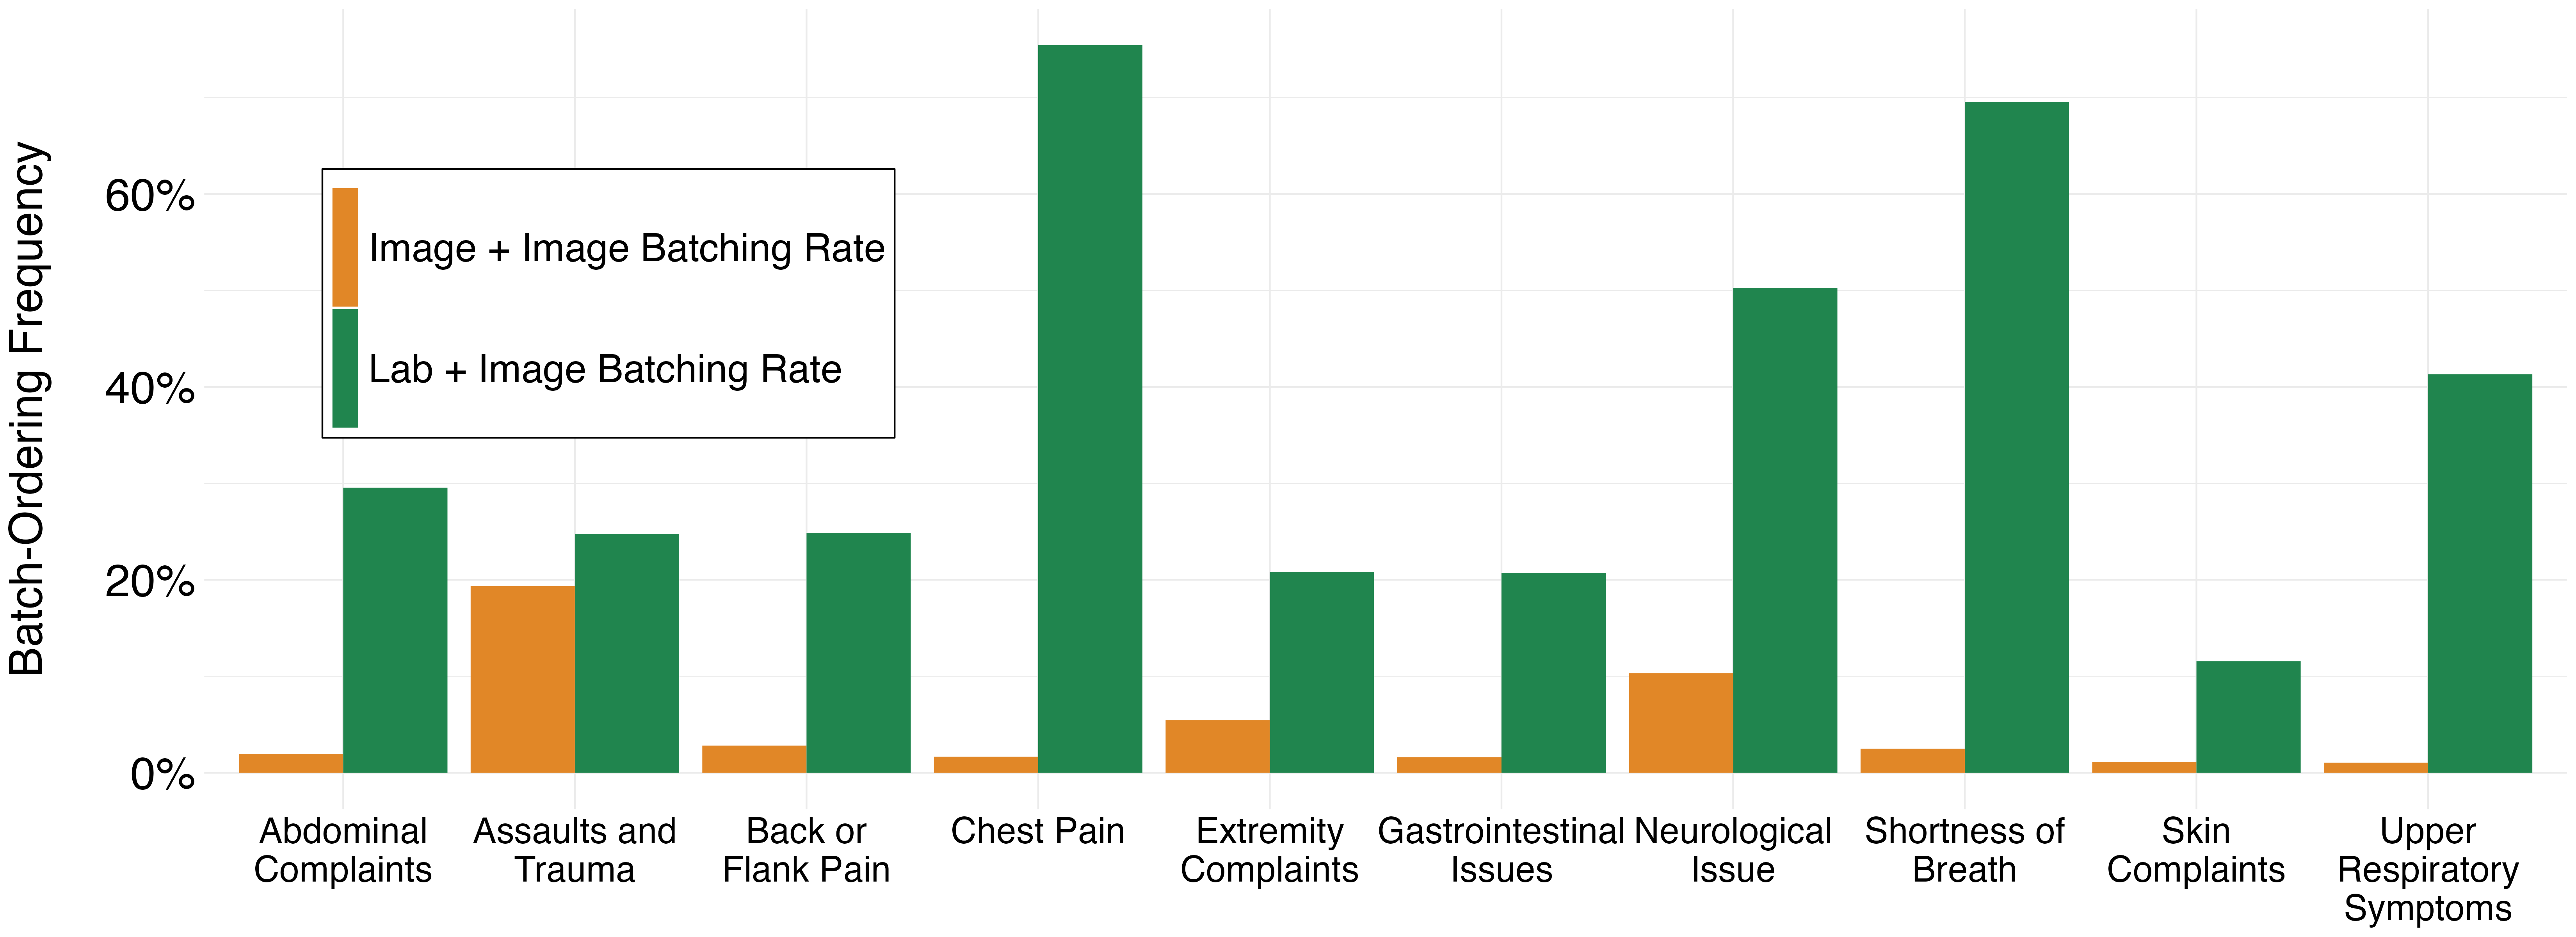
\includegraphics[width=1\textwidth]{../outputs/figures/Lab and Image Batch Rates.png}
\begin{tablenotes}
\small
\item \textit{Figure 1 displays two statistics for the ten most common major chief complaint categories observed in our ED visit sample: the unadjusted batching rate for lab-image batching and image-image batching.}
\end{tablenotes}  
\end{figure}

\hypertarget{summary-statistics}{%
\subsection{Summary Statistics}\label{summary-statistics}}

\hyperref[tab:summary_statistics]{Table 1} presents a detailed overview
of the emergency department (ED) characteristics, patient demographics,
and medical tests for our baseline sample, derived from the data
collected during the study period. On average, the emergency department
manages a volume of approximately 24 patients (Mean = 24.18), indicating
a significant but manageable patient load. Key physiological markers
such as tachycardia (Mean = 0.19) and tachypnea (Mean = 0.09) are
prevalent among patients, albeit at varying degrees, highlighting
critical aspects of emergency care. Notably, a small proportion of
patients exhibit febrile (Mean = 0.02) and hypotensive (Mean = 0.01)
conditions, emphasizing the diversity of cases encountered in the ED
setting. The Emergency Severity Index (ESI) averages at 2.78, suggesting
that most cases fall within the moderate acuity level.

Common chief complaints in the emergency department paint a vivid
picture of patient needs and healthcare demands. The data reveals
abdominal complaints (Mean = 0.14), extremity complaints (Mean = 0.12),
and chest pain (Mean = 0.08) as the most frequently occurring, followed
by neurological (Mean = 0.08) and gastrointestinal issues (Mean = 0.08).
This information is crucial in understanding the primary reasons for ED
visits and the required resources for patient care.

The patient characteristics in our sample depict a diverse demographic
landscape. The average arrival age in the ED is approximately 58 years
(Mean = 58.33), indicating a predominantly middle-aged population. The
racial composition is predominantly White (Mean = 0.89), with smaller
proportions of Black (Mean = 0.04) and Asian (Mean = 0.03) patients.
Notably, a slight majority of the patients are female (Mean = 0.54),
offering insights into gender dynamics in healthcare utilization.

In terms of diagnostic tests, the data reveals a high reliance on lab
tests (Mean = 0.77), indicating their crucial role in patient diagnosis
and management. X-Ray (Mean = 0.47) and CT scans, both non-contrast
(Mean = 0.21) and contrast (Mean = 0.19), are also frequently employed,
underscoring the importance of imaging in modern emergency medicine.
Ultrasound usage (Mean = 0.11) and the practice of batch ordering tests
(Mean = 0.38) further reflect the operational aspects of the ED and the
strategies employed to manage patient care effectively.

\begin{table}[ht]
\centering
\caption{Summary Statistics}
\label{tab:summary_statistics}
\begin{tabular}{p{9cm}cccc}
\toprule
\textbf{} & \textbf{Mean} & \textbf{Q1} & \textbf{Median} & \textbf{Q3} \\
\midrule
\multicolumn{5}{l}{\textbf{ED Characteristics}} \\
ED Volume & 24.18 & 15 & 25 & 32 \\
Tachycardic & 0.19 & & & \\
Tachypneic & 0.09 & & & \\
Febrile & 0.02 & & & \\
Hypotensive & 0.01 & & & \\ 
ESI & 2.78 & 2 & 3 & 3 \\
Complaint: Abdominal & 0.14 & & & \\
Complaint: Extremity & 0.12 & & & \\
Complaint: Chest Pain & 0.08 & & & \\
Complaint: Neurological & 0.08 & & & \\
Complaint: Gastrointestinal & 0.08 & & & \\
\midrule
\multicolumn{5}{l}{\textbf{Patient Characteristics}} \\
Arrival Age & 58.33 & 44 & 62 & 75 \\
Race: White & 0.89 & & & \\
Race: Black & 0.04 & & & \\
Race: Asian & 0.03 & & & \\
Gender: Female & 0.54 & & & \\
\midrule
\multicolumn{5}{l}{\textbf{Tests}} \\
X-Ray & 0.47 & & & \\
Ultrasound & 0.11 & & & \\
Non-Contrast CT & 0.21 & & & \\
Contrast CT & 0.19 & & & \\
Lab & 0.77 & & & \\
Tests were Batch Ordered & 0.38 & & & \\
\bottomrule
\end{tabular}
\begin{tablenotes}
\small
\item \textit{Notes: This table reports summary statistics for the baseline sample of emergency department visits during the study period described in the text.}
\end{tablenotes}
\end{table}

\hypertarget{sec:3}{%
\section{Empirical Strategy}\label{sec:3}}

Our empirical strategy closely follows the literature that relies on
quasi-random assignment of agents to cases, often referred to as the
``judges design.'' Papers in this literature typically exploit variation
in the sentencing leniency of judges who work in the same court.
Similarly, we explore batching variation across physicians who work in
the same emergency department. In its reduced form, under the assumption
of quasi-random assignment, this approach allows researchers to identify
the causal effect of being assigned to different types of physicians.
Under additional assumptions, an instrumental variable approach
identifies the causal effect of a given medical decision. We employ both
approaches and lay out their details in the next subsections.

\hypertarget{institutional-details-on-patient-physician-assignment}{%
\subsection{Institutional Details on Patient-Physician
Assignment}\label{institutional-details-on-patient-physician-assignment}}

Contrary to most healthcare settings where patients exhibit choice, they
are predominantly passive in their physician assignment in the ED. In
most EDs, however, physicians have discretion in picking their patients.
In contrast, patients arriving at the Mayo Clinic ED are randomly
assigned to physicians via a rotational patient assignment algorithm
(Traub et al., 2016), which removes potential selection bias concerns
for our analyses. In essence, barring arrival time and shift-level
variation, the physician-to-patient matching can be deemed random.
\hyperref[tab:summary_statistics]{Table 2} displays that patient
encounters (regarding chief complaints and emergency severity) are
equitably distributed across physicians within our study's cohort.

\begin{table}[htbp]
    \centering
    \caption{Wald Test Results}
    \label{tab:wald_test}
    \begin{tabular}{p{10cm}cc}
        \toprule
        Chief Complaints & F-Statistic & $Pr(> F)$ \\
        \midrule
        Abdominal Complaints & 1.37 & 0.106 \\
        Back or Flank Pain & 1.00 & 0.451 \\
        Chest Pain & 0.98 & 0.476 \\
        Extremity Complaints & 0.97 & 0.495 \\
        Falls, Motor Vehicle Crashes, Assaults, and Trauma & 0.73 & 0.812 \\
        Gastrointestinal Issues & 0.98 & 0.480 \\
        Neurological Issue & 0.75 & 0.793 \\
        Shortness of Breath & 1.23 & 0.199 \\
        Skin Complaints & 1.05 & 0.388 \\
        Upper Respiratory Symptoms & 1.21 & 0.218 \\
        \midrule
        Emergency Severity & F-Statistic & $Pr(> F)$ \\
        \midrule
        ESI 1 or 2 & 1.09 & 0.346 \\
        ESI 3, 4, or 5 & 1.24 & 0.196 \\
        \bottomrule
    \end{tabular}
\begin{tablenotes}
\small
\item \textit{Table 2 reports the results of a Wald test which was conducted to assess the balance of chief complaints across providers in our dataset. A balanced distribution implies that complaints and severity are evenly distributed across providers, which we expect to be the case due to randomization. The Wald F-statistic and p-value are reported. Robust standard errors (type HC1) were used to account for potential heteroscedasticity in the data.}
\end{tablenotes}
\end{table}

\hypertarget{batch-tendency-construction}{%
\subsection{Batch Tendency
Construction}\label{batch-tendency-construction}}

To measure physician batch tendency, we use the physician's residualized
leave-out average batch rate. This measure is derived from two steps
following the approaches taken by \citet{doyle2015measuring},
\citet{dobbie2018effects}, and \citet{eichmeyer2022pathways}. First, we
obtain residuals from a regression model, which includes all ED
encounters in our sample period.

\begin{equation}
Batched_{i,t} = \alpha_0 + \alpha_{ym} + \alpha_{dt} + \alpha_{complaint} + \varepsilon_{i,t}
\end{equation}

Where \(Batched_{i,t}\) is a dummy variable equal to one if patient
\(i\) had their diagnostic tests batched on encounter that took place on
data \(t\). Fixed effects include year-month fixed effects,
\(\alpha_{ym}\), to control for time and seasonal variation in batching,
such as hospital-specific policies (e.g.~initiatives to eliminate excess
testing) or seasonality in ED visits. We also control for
``shift-level'' variations that include both physician scheduling and
patient arrival with day of week-time of day fixed effects,
\(\alpha_{dt}\). Chief complaint by severity fixed effects,
\(\alpha_{complaint}\), were also included to increase precision. As
stated earlier, these controls are what is required for our quasi-random
assignment assumption. Under the assumption that we have captured the
observables under which quasi-random assignment occurs in the ED, the
unexplained variation-- the physician's contribution-- resides in the
error term, \(\varepsilon_{i,t}\).

In step two, the leniency measure for patient \(i\) seen by physician
\(j\) is computed as the average residual across all other patients seen
by the physician that year:

\begin{equation}
Tendency_{i,j}^{phys} =
\frac{1}{N_{-i,j}} \sum_{i' \in \{J \backslash i\}}\hat{\varepsilon}_{i'}
\end{equation}

where \(\hat{\varepsilon}_{i'} = \hat{Batch}_{i'} - Batch_{i'}\) is the
residual from equation (1); \(J\) is the set of all ED encounters
treated by physician \(j\); and \(N_{-i,j} = |\{J \backslash i\}|\), the
number of cases that physician has seen that year, excluding patient
\(i\). This leave-out mean eliminates the mechanical bias that stems
from patient \(i\)'s own case entering into the instrument. The measure
is interpreted as the average (leave-out) batch rate of patient \(i\)'s
physician, relative to other physicians in that hospital-year-month,
hospital-day of week-time of day.

We document that the Mayo Clinic ED physicians exhibit wide, systematic
variation in their propensity to batch order diagnostic tests. Figure 2
graphs the histogram of batch-ordering frequency by physician for
popular chief complaints, highlighting that the variation in batching
differs systematically. \hyperref[tab:regression]{Table 3} presents the
``first stage'' in a regression table: being assigned to a 10 pp higher
tendency physician is associated with a 5 pp increase in the likelihood
of having tests batch-ordered in the ED. The F-statistic is 50 when all
controls and fixed effects are included. The coefficient is greater than
one because all emergency visits are used to construct the leniency
instrument, while the first stage is calculated using the baseline
sample only, which excludes the rare complaints.

\begin{table}[ht]
\centering
\caption{First Stage Regression Results}
\label{tab:regression}
\begin{tabular}{p{9cm}ccc}
\toprule
\textbf{} & \textbf{Model 1} & \textbf{Model 2} & \textbf{Model 3} \\
\midrule
Batching Tendency & 1.05 *** & 1.04 *** & 1.04 *** \\
 & (0.01) & (0.01) & (0.01) \\
\midrule
F statistic (full model) & 7.02 & 50.34 & 49.31  \\  
F (full model): p-value & $<0.001$ & $<0.001$ & $<0.001$ \\
\midrule
Num. obs. & 43327 & 43327 & 43327 \\
Seasonality and shift fixed effects? & Yes & Yes & Yes \\
Chief Complaint? & No & Yes & Yes \\
Patient observables? & No & No & Yes \\
\bottomrule
\end{tabular}
\begin{tablenotes}
\small
\item \textit{Estimates of the first stage for the baseline sample described in the text. Seasonality shift fixed effects include Year-Month and Hospital-Day of week-Hour of day fixed effects. Chief complaint comes from the cleaned complaint that the patient came in with at the initial encounter. Patient observables include sex dummy, race/ethnicity, and age bins. Column 3 corresponds to the baseline controls. Robust standard errors are clustered at the physician level.}
\item $*** p < 0.001$, $** p < 0.01$, $* p < 0.05$.
\end{tablenotes}
\end{table}

To estimate the reduced-form effects of being treated by a
batch-preferring physician, we estimate the following equation:

\begin{equation}
Y_i = \mu_0 + \mu_1 Tendency_{i,j}^{phys} + \gamma X_i + \nu_i
\end{equation}

This reduced form will allow us to check that our instrument is a strong
instrument. To study the effects of test batching in the ED on an
outcome \(Y_i\), we estimate the following 2SLS equations using our
baseline sample:

\begin{equation}
Y_i = \beta_0 + \beta_1 Batched_i + \theta X_i + \varepsilon_i
\end{equation}

\begin{equation}
Batched_i = \delta_0 + \delta_1 Tendency_{i,j}^{phys} + \delta_2 X_i + \nu_i
\end{equation}

Where \(Y_i\) represents our main outcomes of interest: length of stay,
72 hour readmission, and resource utilization. and \(X_i\) is the same
as in the reduced-form approach. \(Batched_i\) variable suffers from
potential endogeneity concerns. For example, injury severity may be
unobserved and correlated with need to run multiple tests, which in turn
also affects length of stay. Hence, we instrument \(Batched_i\) with the
assigned physician \(j\)'s underlying tendency to batch,
\(Tendency_{i,j}^{phys}\) We cluster robust standard errors at the
physician level to account for the assignment process of patients to
physicians.

\hypertarget{identifying-assumptions}{%
\subsection{Identifying Assumptions}\label{identifying-assumptions}}

The reduced-form approach delivers an unbiased estimate of the causal
effect of being treated by a higher tendency to batch physician, since
assignment of patients to ED physicians is random, conditional on
seasonality and shift (``conditional independence''). The
residualization in equation (1) controls for more controls than required
to achieve quasi-random assignment; they are included for statistical
precision in measuring physician tendency to batch.

Our instrumental variable approach, which aims to recover the causal
effect of having diagnostic tests batch ordered, relies on three
additional assumptions: relevance, exclusion, and monotonicity. We
reported a strong first stage (i.e., relevance) at the end of the
previous Section. The exclusion restriction requires that the instrument
must influence the outcome of interest only through its effect on test
batching. This is perhaps our strongest assumption and is at its core,
untestable. However, several features of the ED setting suggest that
such violation may likely only have a small impact and may be less
concerning than in other health care settings. First, unlike in primary
care settings, where the patient and primary care provider have many
repeat encounters, the scope of what the emergency physician can do to
impact medium-term outcomes is limited and well-observed by the
researcher. Second, any violation of the exclusion restriction needs to
directly affect the specific outcome of interest. The channel by which
ED physicians can influence length of stay relative outcomes is likely
through testing and diagnosis. Nevertheless, we take this assumption
seriously and perform a placebo check in Section 4.2 as well as various
robustness checks in Section 4.4.

Finally, the monotonicity assumption is necessary for interpreting the
coefficient estimates obtained from the IV approach as Local Average
Treatment Effects (LATEs) if there are heterogeneous treatment effects.
It requires that any patient who is (not) batched by a sequencer
(batcher) would also (not) be batched by a batcher (sequencer)
physician. The literature leveraging the judges design typically
performs two informal tests for its implications. The first one provides
that the first stage should be weakly positive for all subsamples
(Dobbie, Goldin, and Yang 2018). The second implication asserts that the
instrument constructed by leaving out a particular subsample has
predictive power over that same left-out subsample (Bhuller et
al.~2020). Appendix Table 2 presents both of these tests in the two
columns for various subsamples of interest. Finally, we check whether
our main results hold using differential, mutually exclusive leniency
measures (i.e., by complaint category) in Section 4.4.

\hypertarget{sec:4}{%
\section{Results}\label{sec:4}}

\hypertarget{reduced-form-results}{%
\subsection{Reduced-Form Results}\label{reduced-form-results}}

In this section, we examine the causal effects of provider batching
tendency. Our reduced form regression results, as presented in Table
\ref{tab:reducedform}, indicate that the physician's batch tendency is
associated with longer emergency department length of stay (ED LOS), a
greater number of tests ordered, and does not significantly influence
the likelihood of a 72-hour return. However, the relationship between
batch tendency and our outcomes of interest is nuanced by the presence
of testing inclination among physicians.

\begin{table}[htbp]
\centering
\caption{Reduced Form Regression Results with Scaled Coefficients}
\label{tab:reducedform}
\begin{tabular}{p{6cm}ccc}
\toprule
& \multicolumn{1}{c}{\textbf{Log ED LOS}}
& \multicolumn{1}{c}{\textbf{Number of Tests}}
& \multicolumn{1}{c}{\textbf{72hr Return}} \\
& \multicolumn{1}{c}{(1)}
& \multicolumn{1}{c}{(2)}
& \multicolumn{1}{c}{(3)} \\
\midrule
\textit{Model 1} & & & \\
Batch Tendency      & $0.138^{***}$ & $0.270^{***}$ & $-0.004$  \\
                    & $(0.047)$  & $(0.052)$     & $(0.003)$ \\
\\
Seasonality and shift fixed effects? & Yes & Yes & Yes \\
Chief Complaint? & Yes & Yes & Yes \\
Patient observables? & Yes & Yes & Yes \\
Hospital volume? & Yes & Yes & Yes \\
\midrule
\midrule
\textit{Model 2} & & & \\
Batch Tendency      & $-0.018$      & $0.019^{**}$ & $0.003$   \\
                    & $(0.071)$     & $(0.007)$     & $(0.003)$ \\
                    &     &     &  \\
Testing Inclination    & $0.595^{**}$  & $0.962^{***}$ & $-0.027^{**}$ \\
                    & $(0.234)$  & $(0.021)$     & $(0.011)$ \\
\\
Seasonality and shift fixed effects? & Yes & Yes & Yes \\
Chief Complaint? & Yes & Yes & Yes \\
Patient observables? & Yes & Yes & Yes \\
Hospital volume? & Yes & Yes & Yes \\
\midrule
Mean number of encounters per physician & 1805.3 &  &  \\
\midrule
\bottomrule
\end{tabular}
\begin{tablenotes}
\small
\item \textit{Estimates of the reduced form are for the baseline sample described in the text. Coefficients on batch tendency and testing inclination are scaled by the difference between batch tendency and testing inclination respectively of the ninetieth and tenth percentile physicians for interpretability. Seasonality shift fixed effects include Year-Month and Hospital-Day of week-Hour of day fixed effects. Chief complaint comes from the cleaned complaint that the patient came in with at the initial encounter. Patient observables include sex dummy, race/ethnicity, and age bins. Robust standard errors are clustered at the physician level.}
\item $*** p < 0.001$, $** p < 0.01$, $* p < 0.05$.
\end{tablenotes}
\end{table}

Similar to our method used to measure physician batch tendency, we use
the physician's residualized leave-out average test rate to get a
measure of a physicians propensity to test (which we call testing
inclination). A key consideration in our analysis is the strong positive
correlation (r = 0.79) between batch tendency and testing inclination.
Such a high degree of correlation raises the concern that physicians
with a higher testing inclination may batch more often because as a
result of ordering more tests. Failure to control for this inclination
could result in biased estimates of the effect of batch tendency. We
note this assumption made on the causal pathway and further explore this
in the section on mediation analysis.

In Model 2, we control for testing inclination and observe notable
changes in the coefficients for batch tendency. The previously
significant positive association with Log ED LOS diminishes, suggesting
that the initial estimate may have been capturing the combined effects
of batching and testing inclination. Estimated coefficients for batch
tendency are scaled by the difference in batch tendency going from the
ninetieth to tenth percentile in physician batch tendency---equal to
15.8 pp---for interpretability, and coefficients for testing inclination
are scaled by the difference in testing inclination going from the
ninetieth to tenth percentile in physician testing inclination---equal
to 34.9 pp.

Assignment to a physician in the top batching decile (relative to one in
the bottom decile) is associated with a 0.2 unit increase in the number
of diagnostic tests being ordered per patient encounter, without any
additional change in the liklihood of a 72 hour return. With an average
of 1,805 patient encounters per physician in our study period, this
translates to an additional 8,667 diagnostic tests with no perceived
benefit in terms of reducing returns or length of stay.

The effects of testing inclination are also striking. We find that a
movement from a physician in the top testing decile (relative to one in
the bottom decile) is associated with 0.6\% change in the length of stay
in the emergency department, a 0.96 unit increase in the number of
diagnostic tests being ordered per patient encounter, and -0.03 pp
change in the probability of a patient returning within 72 hours. Given
the average number of patient encounters per physician in our study
period this translates to an additional 1088 patient hours in LOS,
41,594 diagnostic tests, and 47 avoided 72 hour returns.

\hypertarget{placebo-check}{%
\subsection{Placebo Check}\label{placebo-check}}

In this section we investigate whether the reduced-form effects observed
in Section 4.1 are due to differences in batch rates across providers or
due to other provider differences correlated with batch tendency We
start by studying reduced-form effects among patients with complaints
that are never batched, as a ``placebo/falsification check.'' By way of
example, consider a patient who arrives at the ED with a urinary tact
infection---a condition for which patients rarely undergo imaging
testing. For such patients, we should expect to see no impact of batch
tendency only if high batching and low batching physicians do not
systematically differ in other dimensions of care relevant to patient
outcomes. Conversely, if we do find a reduced-form effect for these
patients, then high batch tendency physicians must systematically differ
from low batch tendency physicians in other dimensions of care, beyond
batching.

To that end, we restrict attention to ED visits for complaints where
batching occurs no more than 10 percent of the time (recall that our
baseline sample only includes complaints with a \textgreater10 percent
batching rate). We estimate a reduced-form regression of each main
outcome on physician prescribing leniency for the subsample, following
equation (3). The results of this exercise are displayed in Table \_\_.
They show that in contrast to results for our main sample, the
association between physician tendency to batch and a given outcome is
statistically indistinguishable from zero and much smaller in magnitude
for the samples of patients who visit the ED with health conditions that
are rarely batched.

\hypertarget{instrumental-variables-results}{%
\subsection{Instrumental Variables
Results}\label{instrumental-variables-results}}

\begin{table}[!htbp] \centering 
  \caption{IV Results} 
  \label{} 
\begin{tabular}{p{6cm}ccc}
\\[-1.8ex]\hline 
\hline \\[-1.8ex] 
\\[-1.8ex] & ln\_ED\_LOS & RTN\_72\_HR & nEDTests \\ 
\\[-1.8ex] & (1) & (2) & (3)\\ 
\hline \\[-1.8ex] 
 Batch & $-$0.097 & 0.019 & 0.113$^{***}$ \\ 
  & (0.435) & (0.020) & (0.043) \\ 
  & & & \\ 
 Testing Inclination & 0.607$^{**}$ & $-$0.027$^{**}$ & 0.964$^{***}$ \\ 
  & (0.238) & (0.011) & (0.020) \\ 
  & & & \\ 
Seasonality and shift fixed effects? & Yes & Yes & Yes \\
Chief Complaint? & Yes & Yes & Yes \\
Patient observables? & Yes & Yes & Yes \\
Hospital volume? & Yes & Yes & Yes \\
\midrule
\textit{N} & 43,328 & 43,328 & 43,328 \\ 
R$^{2}$ & 0.195 & 0.009 & 0.306 \\ 
Adjusted R$^{2}$ & 0.190 & 0.002 & 0.302 \\ 
Residual Std. Error (df = 43061) & 0.498 & 0.187 & 0.818 \\ 
\\
\midrule
\midrule
\bottomrule
\end{tabular}
\begin{tablenotes}
\small
\item \textit{Estimates of the IV model are for the baseline sample described in the text. Coefficients on testing inclination are scaled by the difference between testing inclination of the ninetieth and tenth percentile physicians for interpretability. Seasonality shift fixed effects include Year-Month and Hospital-Day of week-Hour of day fixed effects. Chief complaint comes from the cleaned complaint that the patient came in with at the initial encounter. Patient observables include sex dummy, race/ethnicity, and age bins. Robust standard errors are clustered at the physician level.}
\item $*** p < 0.001$, $** p < 0.01$, $* p < 0.05$.
\end{tablenotes}
\end{table}

\hypertarget{robustness}{%
\subsection{Robustness}\label{robustness}}

\hypertarget{conclusion}{%
\section{Conclusion}\label{conclusion}}

\clearpage

\begin{APPENDIX}{General appendix}

\begin{longtable}{|p{5cm}|p{12cm}|}
\caption{Chief Complaints} \\
\hline
\textbf{Complaint Area} & \textbf{Complaints} \\
\hline
Abdominal Complaints & Abdominal Cramping, Abdominal Distention, Dyspepsia, Abdominal Pain, Ascites, Hernia, Abdominal Aortic Aneurysm, Abdominal Injury, Pancreatitis, Umbilical Hernia \\
\hline
Abnormal Test Results & Abnormal Lab, Abnormal Potassium, Abnormal Calcium, ECG Changes, Abnormal ECG, Abnormal Test Result, Blood Infection, Acute Renal Failure, Hypocalcemia, Chronic Renal Failure, Pulmonary Embolism, Abnormal X-ray, Hypoglycemic Unawareness, Elevated Blood Pressure, Abnormal Sodium, Hyperglycemia, Hyponatremia, Platelet Disorders, Anemia, Hypoglycemia, Hypertension, Hypotension, Abnormal Chest Imaging, Abnormal Oximetry, Abnormal Stress Test, Blood Sugar Problem, Hypocalcemia, Hyponatremia \\
\hline
Allergic Reaction & Allergic Reaction, Anaphylaxis \\
\hline
Back or Flank Pain & Back Pain, Back Problem, Flank Pain, Sciatica, Back Injury, Disc Disorder \\
\hline
Breast Complaints & Breast Mass, Breast Pain, Breast Problem, Breast Discharge, Breast Cancer, Breast Discharge, Breast Inflammation \\
\hline
Cardiac Arrhythmias & Atrial Fibrillation, Atrial Flutter, Cardiac Valve Problem, Bradycardia, Irregular Heart Beat, Palpitations, POTS, Ventricular Tachycardia, Rapid Heart Rate, Heart Problem, Cardiac Arrest, Congestive Heart Failure, Circulatory Problem, Transient Ischemic Attack, Ventricular Tachycardia \\
\hline
Chest Pain & Chest Injury, Chest Pain, Chest Wall Pain, Angina, Collarbone Injury, Rib Injury, Heart Pain \\
\hline
Dizziness / Lightheadedness / Syncope & Dizziness, Near Syncope, Syncope, Vertigo, Spells, Hypotension, Paroxysmal Positional Vertigo, Paroxysmal Positional Vertig \\
\hline
Ear Complaints & Cerumen Impaction, Ear Drainage, Ear Fullness, Ear Laceration, Ear Problem, Earache, Hearing Problem, Tinnitus, Ear Injury, Hearing Loss, Nasal Trauma \\
\hline
Epistaxis & Epistaxis, Epistaxis (Nose Bleed), Nose Problem \\
\hline
Exposures, Bites, and Envenomations & Animal Bite, Body Fluid Exposure, Chemical Exposure, Poisoning, Exposure to STD, Insect Bite, Smoke Inhalation, Radiation, Snake Bite, Toxic Inhalation \\
\hline
Extremity Complaints & Ankle Injury, Ankle Pain, Arm Injury, Arm Pain, Cold Extremity, Arm Swelling, Arthritis, Elbow Injury, Elbow Pain, Pseudogout, Extremity Pain, Extremity Weakness, Finger Injury, Hip Injury, Extremity Weakness, Finger Injury, Finger Pain, Dislocation, Foot Infection, Foot Injury, Foot Numbness, Foot Pain, Foot Swelling, Foot Ulcer, Foot Wound Check, Hand Injury, Hand Pain \\
\hline
Eye Complaints & Blurred Vision, Decreased Visual Acuity, Diplopia, Detached Retina, Eye Drainage, Eye Exposure, Eye Pain, Eye Problem, Eye Swelling, Eye Trauma, Foreign Body Eye, Flashes / Light, Loss of Vision, Red Eye, Visual Field Change, Eyelid Problem, Itchy Eye, Eye Exam, Burning Eyes, Eye Twitching, Eyelid/brow Lift Evaluation, Strabismus, Glaucoma, Spots / Floaters \\
\hline
Falls, Motor Vehicle Crashes, Assaults, and Trauma & Assault Victim, Concussion, Facial Injury, Fall, Nasal Trauma, Head Injury, Head Laceration, Motor Vehicle Crash, Puncture Wound, Sexual Assault, Trauma, Domestic Violence, Gun Shot Wound, Work Related Injury, Motorcycle Crash, Injury, Bicycle Accident, Near Drowning, Lip Laceration \\
\hline
Fatigue and Weakness & Difficulty Walking, Fatigue, Gait Problem, Weakness-Generalized, Chronic Fatique, Weakness- Generalized \\
\hline
Fevers, Sweats or Chills & Chills, Diaphoresis, Fever, Night Sweats, Diaphoretic, Diapohresis, Hoarseness, Laryngitis \\
\hline
Foreign Body & Food Bolus, Foreign Body, Foreign Body in Ear, Foreign Body in Skin, Foreign Body in Vagina, Swallowed Foreign Body, Foreign Body in Nose, Foreign Body, FB eye, Foreign Body in Rectum \\
\hline
Gastrointestinal Issues & Anal Fissure, Black or Bloody Stool, Constipation, GERD, Anal Fistula, Diarrhea, Dysphagia, Fecal Impaction, Fistula Follow Up, GIbleeding, GI Problem, Hemorrhoids, Morning Sickness, Nausea, Ostomy Care, Rectal Bleeding, Rectal Pain, Vomiting, Vomiting Blood, Vomiting During Pregnancy, GI Bleeding, Fecal Incontinence, Bloated, Hematochezia, Urine Leakage, Heartburn, Rectal Discharge, Urolithiasis, Ulcerative Colitis, Irritable Bowel Syndrome, Rectal Prolapse, Fistula Evaluation, Rectal Problems, Perianal Abscess, Fisula Evaluation, Stoma Dysfunction \\
\hline
Genital Complaints & Groin Burn, Groin Pain, Groin Swelling, Inguinal Hernia, Menstrual Problem, Pelvic Pain, Penis Pain, Priapism, Testicle Pain, Menorrhagia, Vaginal Bleed, Vaginal Bleeding, Vaginal Itching, Bartholin's Cyst, Genital Warts, Groin Injury, Vaginal Bleeding-Pregnant, Vag Bleed Pregnant, Female Genital Issue, Penis Injury, Vaginal Discharge, Vaginal Pain, Erectile Dysfunction, Vaginal Prolapse, Urethral Stricture, Penile Discharge, Menorrhagia, Gynecologic Exam, Menstrual Problem, Vaginitis/Bacterial Vaginosis, Ovarian Cyst, Vaginitis / Bacterial Vaginosi \\
\hline
Medical Device or Treatment Issue & Cast Problem, Device Check, Dressing Change, Feeding Tube, AICD Problem, Insulin Pump Visit, Gastrostomy Tube Change, Medication Reaction, Shunt, Appliance Removal, Tube Problem, Urinary Catheter Change, Vascular Access Problem, Enteral Nutrition Evaluation, Device Malfunction, Pacemaker Problem, Remova /  Exchange Catheter, Drain Removal, Outpatient Infusion, Treatment, Heart Assist Device, Stoma Dysfunction, Tracheostomy Tube Change, Ureteral Stent Exchange \\
\hline
Medication Request & Immunizations, Infusion / Injection Administration, IV Medication, Infusion/ Injection Administ, Med Refill, Medication Visit, Pain Management, Blood Product Administration, Labs Only, Tetanus (Td \& Tdap), Wound Care \\
\hline
Neurological Issue & Altered Mental Status, Cognitive Concerns, Facial Droop, Pre Syncope, Focal Weakness, Headache, Memory Loss, Migraine, Dementia, Dysphasia, Neuro Problem, Numbness, Paralysis, Seizures, Slurred Speech, Spasms, Stroke Like Symptoms, Tingling, Tremors, Trigeminal Neuralgia, Unable to Speak, Seizure Disorder, Insomnia, Parkinson's Disease, Loss of Consciousness, Neuropathy, Ataxia, Unable to speak, Peripheral Neuropathy, Stroke, Cerebrovascular Accident, Speech Problem, Acute Neurological Problem, Flashes, Light, Unresponsive, Multiple Sclerosis, Parkinson's Disease, Febrile Seizure, Paresthesia, Peripheral Neuropathy, Hydrocephalus, Spasticity, Neuroendocrine Tumor \\
\hline
Other & Dehydration, Fisula Evaluation, Follow-Up, Illness, Letter for School/Work, Aneurysm, Lung Eval, Error, Mass, Oral Swelling, Other, Advice Only, Deformity, Electric Shock, Personal Problem, Shaking, Swelling, Swollen Glands, Adenopathy, Adrenal Problem, Thrombophilia, Weight Gain, Weight Loss, Hiccups, , Chemo Related Symptoms, Hot Flashes, Follow-up, Non Healing Wound, (Other), Mouth Injury, Xerostomia, Prostate Check, Suture / Staple Removal, Wellness, Voice Changes, Vital Sign Check, Coagulation Disorder, Cold Exposure, Consult, Dental Problem, Tetanus (Td \& Tdap), Infusion/ Injection Administ, Tracheostomy Tube Change, Medical Information, Neutropenic Fever, Infection, Leukemia, Heat Exposure, Poor Appetite, Gingivitis, Pre-op Exam, gingivitis, Loss of appetite, Failure To Thrive, Referral, Lymphoma, Hot Flashes, Neutropenia, Radiation, Ingestion, TB Test, Fussy, Lupus, Toxic Inhalation, Lung Screening, Leakage/Loss of Fluid, Liver Eval, Hepatic Cancer, Lung Mass, Venous Thromboembolic Disease, Insulin Pump Visit, Preventive Visit, Avulsion, Peripheral Edema, Hypoglycemic Unawareness, Immobility, Giant Cell Arteritis, Polydipsia, Platelet Disorders, Post-procedure, Lung Follow-up, Poisoning, Injections, POTS, Insulin Reaction, Liver Transplant, Labs Only \\
\hline
Other Pain & Dental Pain, Facial Pain, Generalized Body Aches, Myalgia, Dental Injury, Jaw Pain, Muscle Pain, Neck Pain, Pain, Sickle Cell Pain Crisis, Paresthesia, Torticollis, Chronic Pain, Cancer Pain, Incisional Pain, Bone Pain, Tailbone Pain, Gout, Muscle pain/Weakness, Pseudogout \\
\hline
Post-Op Issue & Post-Op, Post-Procedure, Post-Op Problem, Post-op, Post-Op Issue, Wound Dehiscence, Post-op Problems, Post-op Problem \\
\hline
Psychiatric Complaints & Anxiety, Auditory Hallucinations, Depression, Panic Attack, Homicidal, PTSD (Post-Traumatic Stress, Delusional, Fussy, Paranoia, Suicide Attempt, Hallucinations, Manic Behavior, Eating Disorder, Suicidal, Agitation, Psychiatric Evaluation, Aggressive Behavior, Mental Health Problem, Inappropriate Words \\
\hline
Shortness of Breath & Airway Obstruction, Aspiration, Pain With Breathing, Near Drowning, Respiratory Distress, Shortness of Breath, Wheezing, Increased Work Of Breathing, Difficulty Breathing, Choking, Oxygen Dependence, Hyperventilating, Orthopnea \\
\hline
Skin Complaints & Abrasion, Abscess, Bleeding/Bruising, Blister, Angioedema, Lip Laceration, Burn, Cellulitis, Cyst, Drainage from Incision, Disturb of Skin Sens, Edema, Extremity Laceration, Facial Burn, Cyanosis, Impetigo, Facial Laceration, Facial Swelling, Finger Laceration, Leg Rash, Herpes Zoster, Hives, Itching, Jaundice, Diabetic Ulcer, Diabetic Wound, Laceration, Mouth Lesions, Non-Healing Wound, Rash, Recurrent Skin Infections, Skin Problem, Sore, Scabies, Suture \textbackslash Staple Removal, Wound Check, Wound Infection, Lesion, Skin Check, Minor Skin Infection, Skin Ulcer, Skin Discoloration, Sunburn, Head Lice, Scabies, Fungal Infection, Leg Rash, Impetigo \\
\hline
Substance Abuse Issues & Alcohol Intoxication, Alcohol Problem, Withdrawal, Drug Overdose, Drug / Alcohol Dependency, Addiction Problem, Addiction Assessment, Delirium Tremens (DTS) \\
\hline
Upper Respiratory Symptoms & Congestion, Cough, Coughing Up Blood, Flu Symptoms, Enlarged Tonsils, Peritonsillar Abscess, Nasal Congestion, Sinus Symptoms, Sinusitis, Sore Throat, Hoarseness, Throat Problem, Upper Respiratory Infection, Influenza, Laryngitis, Respiratory Arrest, Pneumonia, Pleural Effusion, Asthma, Croup, URI, Peritonsillar Abscess \\
\hline
Pregnancy Related & Pregnancy Problem, Miscarriage, Contractions, Ectopic Pregnancy, Laboring, Possible Pregnancy, Pregnancy Related \\
\hline
Renal & Av Fistula, Kidney Transplant, Elevated Serum Creatinine, End-Stage Liver Disease, Hemodialysis Access, Nephritis, Ureteral Stent Exchange \\
\hline
Urinary Complaints & Bladder Problem, Blood in Urine, Cystitis, Difficulty Urinating, Dysuria, Gross Hematuria, Painful Urination, Urinary Frequency, Urinary Symptom, Urinary Incontinence, Urinary Problem, Urinary Retention, Slowing Urinary Stream, Urinary Tract Infection, Urinary Urgency, Voiding Dysfunction, Hesitancy Urinary \\
\hline
\end{longtable}

\end{APPENDIX}

% Appendix here
% Options are (1) APPENDIX (with or without general title) or
%             (2) APPENDICES (if it has more than one unrelated sections)
% Outcomment the appropriate case if necessary
%
% \begin{APPENDIX}{<Title of the Appendix>}
% \end{APPENDIX}
%
%   or
%
% \begin{APPENDICES}
% \section{<Title of Section A>}
% \section{<Title of Section B>}
% etc
% \end{APPENDICES}


% Acknowledgments here
\ACKNOWLEDGMENT{The authors would like to thank ..}

\bibliographystyle{informs2014}
\bibliography{references.bib}



\end{document}
